\documentclass[fleqn]{jbook}
\usepackage{physpub}

\begin{document}

\begin{question}{$B@l96(B $BLdBj(B1}{$BC]0fMN(B(s91546)}
\parbox[t]{.5\linewidth}{
$B?^(B1$B$N$h$&$J(B1$B<!85%]%F%s%7%c%k(B$V(x)$$B$9$J$o$A(B
\begin{eqnarray*}
V(x) &=& \infty \qquad \text{($\Norm{x}>d+a$$B$N$H$-(B),} \\
V(x) &=& 0 \qquad \text{($d+a>\Norm{x}>d$$B$N$H$-(B),} \\
V(x) &=& V_0 \qquad \text{($\Norm{x}<d$$B$N$H$-(B),}
\end{eqnarray*}
$B$NCf$K<ANL(B$m$$B$NN3;R$,0l8DF~$C$F$$$k7O$r9M$($k!#$3$N$h$&$K!"(B1$B<!85%7%e%l%G%#%s%,!<J}Dx<0$G%]%F%s%7%c%k%(%M%k%.!<$,(B1$B<!85:BI8(B$x$$B$N4X?t$H$7$F(B$V(x)=V(-x)$$B$rK~$?$9$H$-!"%O%_%k%H%K%"%s(B
\[ H(x)=-\frac{\hbar}{2m}\frac{\d{}^2}{\d{x}^2}+V(x) \]
}
\parbox[t]{.5\linewidth}{
\vspace*{-1cm}
\begin{center}
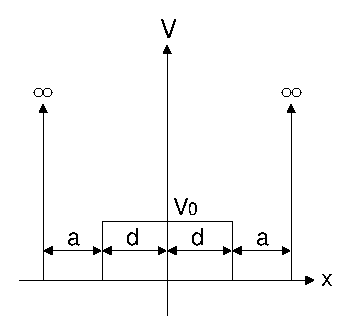
\includegraphics[clip]{1999phy1-1.eps}\\
$B?^(B1
\end{center}
}
$B$N8GM-4X?t(B$\Psi$$B$O(B$\Psi(x)=\Psi(-x)$$B$G$"$k%Q%j%F%#$,6v$N$b$N$H(B$\Psi(x)=-\Psi(-x)$$B$G$"$k%Q%j%F%#$,4q$N$b$N$KJ,$+$l$k$3$H$KCm0U$7$F!"0J2<$NLd$$$KEz$($h!#C"$7(B$\hbar$$B$O%W%i%s%/Dj?t$G$"$k!#(B


\begin{subquestions}

\SubQuestion

$B$3$N7O$N%(%M%k%.!<8GM-CM(B$E$$B$r7h$a$k<0$r(B$E<V_0$$B$N>r7o$,K~$?$5$l$F$$$k>l9g$K$D$$$F5a$a$h!#(B

\SubQuestion

$B4pDl>uBV$HBh0lNe5/>uBV$NGHF04X?t$r$=$l$>$l(B$\Ket{\Psi_0}$$B$H(B$\Ket{\Psi_1}$$B$H$7!"%(%M%k%.!<8GM-CM$r$=$l$>$l(B$E=E_0,E_1$$B$H$9$k!#(B$E_1<V_0$$B$,K~$?$5$l$k>l9g$K!"(B$\Ket{\Psi_0}$$B$H(B$\Ket{\Psi_1}$$B$N357A$r(B$x$$B$N4X?t$H$7$FIA$1!#(B

\SubQuestion

$V_0$$B$,M-8B$G(B$d$$B$,L58BBg$N6K8B$r$H$C$?;~$N(B$E_0,E_1$$B$r(B$\overline{E_0},\overline{E_1}$$B$H$9$k!#(B$\overline{E_0},\overline{E_1}$$B$r0l0UE*$K7h$a$k<0$r5a$a$h!#(B

\SubQuestion

$d$$B$,Bg$-$$$,M-8B$G$"$k$H$9$k!#(B$\overline{E_0}$$B$rMQ$$$F!"(B$\Delta\equiv E_1-E_0$$B$N(B$d$$B0MB8@-$,$I$&$J$C$F$$$k$+$r5DO@$;$h!#(B
\end{subquestions}

$V_0$$B$H(B$d$$B$,Bg$-$$$H$-!"5,3J2=$5$l$?GHF04X?t(B$\Ket{\Psi_0}$$B$d(B$\Ket{\Psi_1}$$B$N$[$H$s$I$N=E$_$O(B$d+a>\Norm{x}>d$$B$NCf$K$"$k$H9M$($F$h$$!#$7$?$,$C$F!"(B$\Ket{\Psi_0}$$B$d(B$\Ket{\Psi_1}$$B$O6a;wE*$K1&$N0f8M$KN3;R$,B8:_$7!"$o$:$+$K(B$\Norm{x}<d$$B$X?;$_=P$7$F$$$k>uBV(B$\Ket{R}$$B$H!":8$N0f8M$KN3;R$,B8:_$7!"$o$:$+$K(B$\Norm{x}<d$$B$X?;$_=P$7$F$$$k>uBV(B$\Ket{L}$$B$N(B1$B<!7k9g$G$"$i$o$5$l$k$H$_$J$;$k!#(B$\Ket{R}$$B$H(B$\Ket{L}$$B$O5,3J2=$5$l!"8_$$$KD>8r$7$F$$$k$H$7!"$^$?!"(B$\Ket{\Psi_0}$$B$d(B$\Ket{\Psi_1}$$B$h$j$b9b$$Ne5/>uBV$K$D$$$F$OL5;k$7$FNI$$$H$7$F!"0J2<$KEz$($h!#(B

\begin{subquestions}[5]

\SubQuestion

$\Ket{\Psi_0}$$B$H(B$\Ket{\Psi_1}$$B$r(B$\Ket{R}$$B$H(B$\Ket{L}$$B$N(B1$B<!7k9g$GI=$;!#(B

\SubQuestion

$\Ket{R}$$B$H(B$\Ket{L}$$B$r4pDl$H$9$kI=8=$r$H$C$F!"%O%_%k%H%K%"%s$r(B2$B9T(B2$BNs$N9TNs$GI=$;!#(B

\SubQuestion

$t=0$$B$KN3;R$NGHF04X?t$,1&$N0f8M$KB8:_$9$k>uBV(B$\Ket{R}$$B$GI=$o$5$l$F$$$?$H$-!"%H%s%M%j%s%0$K$h$C$F;~9o(B$t$$B$KN3;R$,:8$N0f8M$N>uBV(B$\Ket{L}$$B$K0\$C$F$$$k3NN($r(B$\Delta$$B$rMQ$$$FI=$o$7!"F@$i$l$?(B$\Delta$$B0MB8@-$NJ*M}E*0UL#$r5DO@$;$h!#(B

\end{subquestions}
\end{question}
\begin{answer}{$B@l96(B $BLdBj(B1}{$BC]0fMN(B(s91546)}
\begin{subanswers}

\SubAnswer
$\Psi_{\pm}(x)=\pm\Psi_{\pm}(-x)$$B$N$h$&$J2r$,$"$k!#(B
\begin{itemize}
\item[(i)]
~$0\le x \le d$$B$N$H$-(B

\begin{gather*}
-\frac{\hbar^2}{2m}\Psi_{1\pm}''(x)+V_0\Psi_{1\pm}(x)=E_{\pm}\Psi_{1\pm}(x) \\
\alpha_{\pm}\equiv\frac{\sqrt{2m(V_0-E_{\pm})}}{\hbar}\;  \text{$B$H$7$F(B} \\
\Psi_{1\pm}(x)=Ae^{\alpha_{\pm} x}+Be^{-\alpha_{\pm} x} \\
\end{gather*}

\begin{itemize}

\item[\textbullet] ~parity even$B$N$H$-(B
\begin{gather*}
\Psi_{1+}(x)=\Psi_{1+}(-x)\; \text{$B$h$j(B} \; A=B \\
\therefore \Psi_{1+}(x)=A_+\cosh (\alpha_+ x) \\
\end{gather*}

\item[\textbullet] ~parity odd$B$N$H$-(B
\begin{gather*}
\Psi_{1-}(x)=-\Psi_{1-}(-x)\; \text{$B$h$j(B} \; A=-B \\
\therefore \Psi_{1-}(x)=A_-\sinh (\alpha_- x) \\
\end{gather*}

\end{itemize}

\item[(ii)]
~$d\le x \le d+a$$B$N$H$-(B
\begin{gather*}
-\frac{\hbar^2}{2m}\Psi_{2\pm}''(x)=E_{\pm}\Psi_{2\pm}(x) \\
\beta_{\pm}\equiv \frac{\sqrt{2mE_\pm}}{\hbar}\; \text{$B$H$7$F(B}\\
\Psi_{2\pm}(d+a)=0\text{$B$N6-3&>r7o$h$j(B}\\
\Psi_{2\pm}(x)=B_{\pm}\sin\left(\beta_\pm(x-a-d)\right) \\
\text{$B$H=q$1$k!#(B}
\end{gather*}

\end{itemize}
$B$3$l$i$+$i(B$E$$B$r5a$a$k!#(B

\begin{itemize}

\item ~parity even$B$N$H$-(B

\begin{gather*}
\begin{cases}
\Psi_{1+}(x)=A_+\cosh\alpha_+x \\
\Psi_{2+}(x)=B_+\sin\left(\beta_+(x-a-d)\right)
\end{cases}
\\
\text{$B6-3&>r7o$h$j(B}
\\
\begin{cases}
\Psi_{1+}(d)=\Psi_{2+}(d) \\
\Psi'_{1+}(d)=\Psi'_{2+}(d)
\end{cases}
\\
\text{$B$7$?$,$C$F(B}
\\
\begin{cases}
A_+\cosh\alpha_+d=-B_+\sin\beta_+a \\
A_+\alpha_+\sinh\alpha_+d=B_+\beta_+\cos\beta_+a
\end{cases}
\\
\therefore \alpha_+\tanh\alpha_+d=-\beta_+\cot\beta_+a
\end{gather*}

$B$3$l$K$h$j(B$E$$B$,5a$^$k!#(B

\item ~parity odd$B$N$H$-(B

\begin{gather*}
\begin{cases}
\Psi_{1-}(x)=A_-\sinh\alpha_-x \\
\Psi_{2-}(x)=B_-\sin\left(\beta_-(x-a-d)\right)
\end{cases}
\\
\text{$B6-3&>r7o$h$j(B}
\\
\begin{cases}
\Psi_{1-}(d)=\Psi_{2-}(d) \\
\Psi'_{1-}(d)=\Psi'_{2-}(d)
\end{cases}
\\
\text{$B$7$?$,$C$F(B}
\\
\begin{cases}
A_-\sinh\alpha_-d=-B_-\sin\beta_-a \\
A_-\alpha_-\cosh\alpha_-d=B_-\beta_-\cos\beta_-a
\end{cases}
\\
\therefore \frac{1}{\alpha_-}\tanh\alpha_-d=-\frac{1}{\beta_-}\tan\beta_-a
\end{gather*}

$B$3$l$K$h$j(B$E$$B$,5a$^$k!#(B

\end{itemize}

\SubAnswer

parity even$B$N$H$-!#(B
\begin{center}
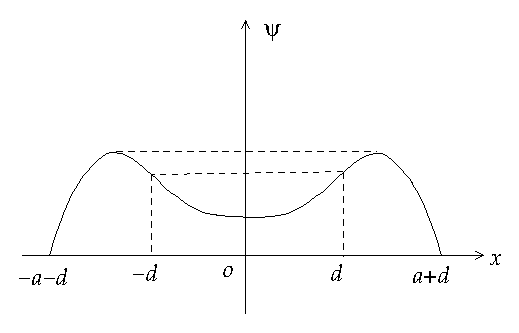
\includegraphics[clip]{1999phy1-2.eps}
\end{center}

parity odd$B$N$H$-!#(B
\begin{center}
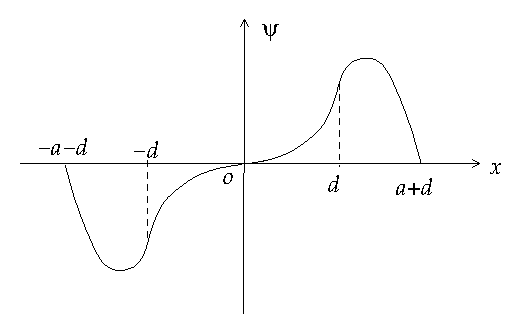
\includegraphics[clip]{1999phy1-3.eps}
\end{center}

\SubAnswer
$d\rightarrow\infty$$B$G$O(B
\[ \tan\beta_{\pm}a=-\frac{\beta_{\pm}}{\alpha_{\pm}} \]
$B$h$j!"%(%M%k%.!<=`0L$O=LB`$7$F$$$F(B
\[ \overline{E_0}=\overline{E_1} \]
$B%(%M%k%.!<$NCM$b$3$N<0$h$j5a$^$k!#(B

\SubAnswer

\begin{align*}
\tanh\alpha x &= \frac{e^{\alpha x}-e^{-\alpha x}}{e^{\alpha x}+e^{-\alpha x}} \\
&= \frac{1-e^{-2\alpha x}}{1+e^{-2\alpha x}}
\end{align*}
$x$$B$,==J,Bg$-$$$H$9$k$H(B
\begin{align*}
\tanh\alpha x &\sim \left(1-e^{-2\alpha x}\right)^2 \\
&\sim 1-2e^{-2\alpha x}
\end{align*}
$B$7$?$,$C$F(B
\[ \tan\beta_{\pm}a=-\frac{\beta_{\pm}}{\alpha_{\pm}}\mp 2\frac{\beta_{\pm}}{\alpha_{\pm}}e^{-2\alpha_{\pm}d} \]
\begin{gather*}
\alpha_0\equiv\frac{\sqrt{2m(V_0-E_0)}}{\hbar}\; ,\;\beta_0\equiv \frac{\sqrt{2mE_0}}{\hbar}\;\text{$B$H$9$k$H(B}\\
\beta_{\pm}a=\pi-\frac{\beta_0}{\alpha_0}\left(1\pm2e^{-2\alpha_0 d}\right)
\end{gather*}

$\beta_+$$B$O4pDl>uBV!"(B$\beta_-$$B$OBh0lNe5/>uBV$H$J$k$N$G(B
\[ \Delta\equiv E_1-E_0=\frac{\hbar^2}{2m}\left(\beta_-^2-\beta_+^2\right) \quad \cdots \quad \propto e^{-2\alpha_0d} \]
$B$h$C$F!"(B$\Delta$$B$O(B$d$$B$K;X?t4X?tE*$K0MB8$7$F$$$k!#(B

\SubAnswer

\begin{align*}
\Ket{\Psi_0}&=\frac{1}{\sqrt{2}}\Bigl( \Ket{R}+\Ket{L}\Bigr) \\
\Ket{\Psi_1}&=\frac{1}{\sqrt{2}}\Bigl( \Ket{R}-\Ket{L}\Bigr)
\end{align*}

\SubAnswer

\begin{align*}
\Ket{R}&=\frac{1}{\sqrt{2}}\Bigl( \Ket{\Psi_0}+\Ket{\Psi_1}\Bigr) \\
\Ket{L}&=\frac{1}{\sqrt{2}}\Bigl( \Ket{\Psi_0}-\Ket{\Psi_1}\Bigr)
\end{align*}

\begin{align*}
\Bracket{R}{H}{R} &= \frac{1}{2}\Bigl(\Bra{\Psi_0}+\Bra{\Psi_1}\Bigr)\Bigl(E_0\Ket{\Psi_0}+E_1\Ket{\Psi_1}\Bigr)
= \frac{E_0+E_1}{2} \\
\Bracket{L}{H}{L} &= \frac{1}{2}\Bigl(\Bra{\Psi_0}-\Bra{\Psi_1}\Bigr)\Bigl(E_0\Ket{\Psi_0}-E_1\Ket{\Psi_1}\Bigr)
= \frac{E_0+E_1}{2} \\
\Bracket{R}{H}{L} &= \frac{1}{2}\Bigl(\Bra{\Psi_0}+\Bra{\Psi_1}\Bigr)\Bigl(E_0\Ket{\Psi_0}-E_1\Ket{\Psi_1}\Bigr)
= -\frac{E_1-E_0}{2}
= -\frac{\Delta}{2} \\
\Bracket{L}{H}{R} &= \frac{1}{2}\Bigl(\Bra{\Psi_0}-\Bra{\Psi_1}\Bigr)\Bigl(E_0\Ket{\Psi_0}+E_1\Ket{\Psi_1}\Bigr)
= -\frac{E_1-E_0}{2}
= -\frac{\Delta}{2} \\
\end{align*}
\[ 
\therefore H \doteq
\begin{pmatrix}
\cfrac{E_0+E_1}{2} & -\cfrac{\Delta}{2} \\
-\cfrac{\Delta}{2} & \cfrac{E_0+E_1}{2}
\end{pmatrix}
\]
\\


\SubSubAnswer
Schr\"{o}dinger$BI=<($G9M$($k!#(B

\begin{gather*}
H\Ket{R(t)}=i\hbar\frac{\del}{\del t}\Ket{R(t)}\; ,\; \Ket{R(0)}=\Ket{R} \\
\therefore \Ket{R(t)}=e^{-iHt/\hbar}\Ket{R}
\end{gather*}

\begin{align*}
e^{-iHt/\hbar} &\doteq \sum_k\frac{(-it/\hbar)^k}{k!}
\begin{pmatrix}
\frac{E_0+E_1}{2} & -\frac{\Delta}{2} \\
-\frac{\Delta}{2} & \frac{E_0+E_1}{2}
\end{pmatrix}
^k \\
&= \sum_k\frac{1}{k!}\frac{(-it/\hbar)^k}{2}
\begin{pmatrix}
E_0^k+E_1^k & E_0^k-E_1^k \\
E_0^k-E_1^k & E_0^k+E_1^k 
\end{pmatrix}
\\
&= \frac{1}{2}
\begin{pmatrix}
e^{-iE_0t/\hbar}+e^{-iE_1t/\hbar} & e^{-iE_0t/\hbar}-e^{-iE_1t/\hbar} \\
e^{-iE_0t/\hbar}-e^{-iE_1t/\hbar} & e^{-iE_0t/\hbar}+e^{-iE_1t/\hbar}
\end{pmatrix}
\end{align*}

\begin{align*}
\therefore \Product{L}{R(t)} &= \frac{1}{2}\Bra{L}\left\{ \left(e^{-iE_0t/\hbar}+e^{-iE_1t/\hbar}\right)\Ket{R}+\left(e^{-iE_0t/\hbar}-e^{-iE_1t/\hbar}\right)\Ket{L}\right\} \\
&= \frac{1}{2}\left(e^{-iE_0t/\hbar}-e^{-iE_1t/\hbar}\right)
\end{align*}

\begin{align*}
\therefore \Norm{\Product{L}{R(t)}}^2 &= \frac{1}{4}\left(e^{-iE_0 t/\hbar} - e^{-iE_1 t/\hbar}\right)
\left(e^{iE_0 t/\hbar} - e^{iE_1 t/\hbar}\right)\\
&= \frac{1}{4}\left(2-e^{-i\Delta t/\hbar}-e^{i\Delta t/\hbar}\right)\\
&= \frac{1}{2}\left(1-\cos\frac{\Delta}{\hbar}t \right)\\
&=\sin^2\frac{\Delta}{2\hbar}t
\end{align*}

$B$3$l$h$j!"(B$\Delta$$B$,Bg$-$$!"$D$^$j(B$V_0$$B$d(B$d$$B$,>.$5$$;~$[$IB.$/(B$\Ket{R}\leftrightarrow\Ket{L}$$B$N<~4|E*A+0\$r$9$k$3$H$,$o$+$k!#(B

\end{subanswers}
\end{answer}


\end{document}
